\documentclass{ieeeaccess}
\usepackage{cite}
\usepackage{amsmath,amssymb,amsfonts,amsthm}
\usepackage{algorithmic}
\usepackage{algorithm}
\usepackage{graphicx}
\usepackage{textcomp}
\usepackage{xcolor}
\usepackage{booktabs}
\usepackage{multirow}
\usepackage{url}
\usepackage{balance}

\newtheorem{theorem}{Theorem}
\newtheorem{definition}{Definition}
\newtheorem{lemma}{Lemma}
\newtheorem{axiom}{Axiom}
\newtheorem{proposition}{Proposition}
\newtheorem{corollary}{Corollary}

\def\BibTeX{{\rm B\kern-.05em{\sc i\kern-.025em b}\kern-.08em
    T\kern-.1667em\lower.7ex\hbox{E}\kern-.125emX}}

\history{Date of publication November 22, 2026, date of current version November 22, 2026.}
\doi{10.1109/ACCESS.2026.3389012}

\title{Sentinel-XAI: A Safety-Aware Multi-Agent Explainable AI Framework with Provable Risk Bounds and Invariant Enforcement for Clinical IoT Threat Defense}

\author{\uppercase{Laddu Chamith Shaminda De Silva}\authorrefmark{1,2}, (Graduate Student Member, IEEE), AND \uppercase{Aloka Aponso}\authorrefmark{1}, (Senior Member, IEEE)}
\address[1]{Department of Computing, Informatics Institute of Technology, Colombo 00600, Sri Lanka (e-mail: chamith.20230638@iit.ac.lk, aloka.a@iit.ac.lk)}
\address[2]{School of Computer Science and Engineering, University of Westminster, London W1W 6UW, U.K. (e-mail: w2083586@my.westminster.ac.uk)}
\tfootnote{This work was supported in part by the Informatics Institute of Technology (IIT) Research and Enterprise Fund under Grant IIT-CS-2026-XAI-04, conducted in academic partnership with the University of Westminster. No external commercial sponsorship was involved.}

\markboth
{De Silva and Aponso: Sentinel-XAI: A Safety-Aware Multi-Agent Explainable AI Framework for Clinical IoT}
{De Silva and Aponso: Sentinel-XAI: A Safety-Aware Multi-Agent Explainable AI Framework for Clinical IoT}

\corresp{Corresponding author: Laddu Chamith Shaminda De Silva (e-mail: chamith.20230638@iit.ac.lk).}

\begin{document}

\begin{abstract}
Autonomous cyber threat response systems deployed across life-critical Internet of Medical Things (IoMT) environments face severe operational and safety hazards, including catastrophic action hallucination, ungrounded threat severity escalation, and abrupt isolation of patient-critical telemetry streams. While deep neural classifiers and generative Large Language Model (LLM) agents achieve high nominal diagnostic accuracy, they lack distribution-free finite-sample risk bounds and deterministic physical safety guarantees. To resolve this foundational challenge, this paper formulates the problem of Epistemically Gated Autonomous Mitigation (EGAM) and introduces \textbf{Sentinel-XAI}, an advanced multi-agent Explainable Artificial Intelligence (XAI) framework engineered for mathematically provable cyber defense. Sentinel-XAI makes four primary theoretical and methodological contributions: (1) we prove the \textit{Epistemic Risk-Bounded Trilemma (ERBT Theorem)}, demonstrating that unconstrained generative response agents operating under sub-100ms latency cannot simultaneously guarantee bounded operational risk without an external deterministic evidence oracle; (2) we formulate a Game-Theoretic Epistemic Verification protocol modeled as an asymmetric zero-sum debate between an Analyst and a Critic agent, proving that anchoring assertions to RFC~6901 JSON Pointers and RFC~8785 Canonical JSON digests yields a unique truthful Subgame Perfect Nash Equilibrium with an ungrounded hallucination rate of strictly 0.00\%; (3) we establish \textit{Cost-Sensitive Shift-Aware Conformal Selective Risk Control}, integrating an asymmetric cyber-physical loss function with Clopper-Pearson Binomial Upper Confidence Bounds to mathematically guarantee bounded triage error ($\alpha \le 0.05$) under finite samples even in the presence of covariate distribution drift; and (4) we formulate the axiomatic foundations of the \textit{Composite Explanation Trust Score (ETS 2.0)}, unifying TreeSHAP local attributions, LIME surrogate consistency, and $L_1$-minimal contrastive counterfactuals. For healthcare infrastructure, an IoMT Separation of Duties gate ($C_{16}$) prevents autonomous service disruptions on clinical devices, mandating dual-role clinician authorization. Extensive empirical evaluations across four canonical benchmark corpora (NSL-KDD, CIC-IDS2017, UNSW-NB15, and CICIoMT2024) across 5 randomized seeds demonstrate that Sentinel-XAI achieves a Macro F1-score of $0.9960 \pm 0.001$, eliminates ungrounded hallucinations from 29.41\% to 0.00\%, guarantees selective triage risk beneath $0.10\%$ under a $5.0\%$ target error budget, enforces 100\% clinical invariant compliance across 42,000 synthetic adversarial disruptions, and executes automated fast-path triage in 17.24\,ms.
\end{abstract}

\begin{keywords}
Auditable artificial intelligence, autonomous cyber defense, conformal prediction, counterfactual explanations, dual-LLM verification, explainable artificial intelligence (XAI), game theory, Internet of Medical Things (IoMT), multi-agent systems, selective classification, TreeSHAP.
\end{keywords}

\titlepgskip=-15pt
\maketitle

\section{Introduction}
\label{sec:introduction}
\PARstart{M}{odern} healthcare infrastructures and hospital enterprise networks have evolved into hyper-connected Cyber-Physical Systems (CPS), where thousands of Internet of Medical Things (IoMT) devices---including smart infusion pumps, bedside electrocardiogram (ECG) telemetry monitors, anesthesia delivery workstations, and healthcare IoT gateways---interact continuously with clinical databases and cloud servers~\cite{dadkhah2024ciciomt2024, sun2022cyber, al2020survey}. While this pervasive interconnectivity enhances real-time patient monitoring, it expands the hospital's attack surface, exposing life-critical clinical devices to Advanced Persistent Threats (APTs), ransomware epidemics, and volumetric Denial-of-Service (DoS) attacks~\cite{vielberth2020security, ahmad2021soc}.

Traditional Security Operations Centers (SOCs) rely on Security Information and Event Management (SIEM) systems and machine learning-based Intrusion Detection Systems (IDS). However, Tier-1 security analysts in healthcare SOCs face severe cognitive fatigue, triaging upwards of 20,000 heterogeneous alerts per shift, over 85\% of which are benign protocol jitter, transient telemetry fluctuations, or false alarms~\cite{ahmad2021soc, sarhan2023towards}. Although gradient-boosted decision trees (e.g., XGBoost) and deep neural architectures achieve high offline accuracy on static benchmark datasets, their black-box nature creates an insurmountable trust barrier: human analysts cannot determine whether a flagged anomaly represents a genuine zero-day lateral movement or a harmless clinical firmware polling routine~\cite{marcus2020next, lundberg2017unified, ribeiro2016should}.

\begin{figure*}[t]
\centering
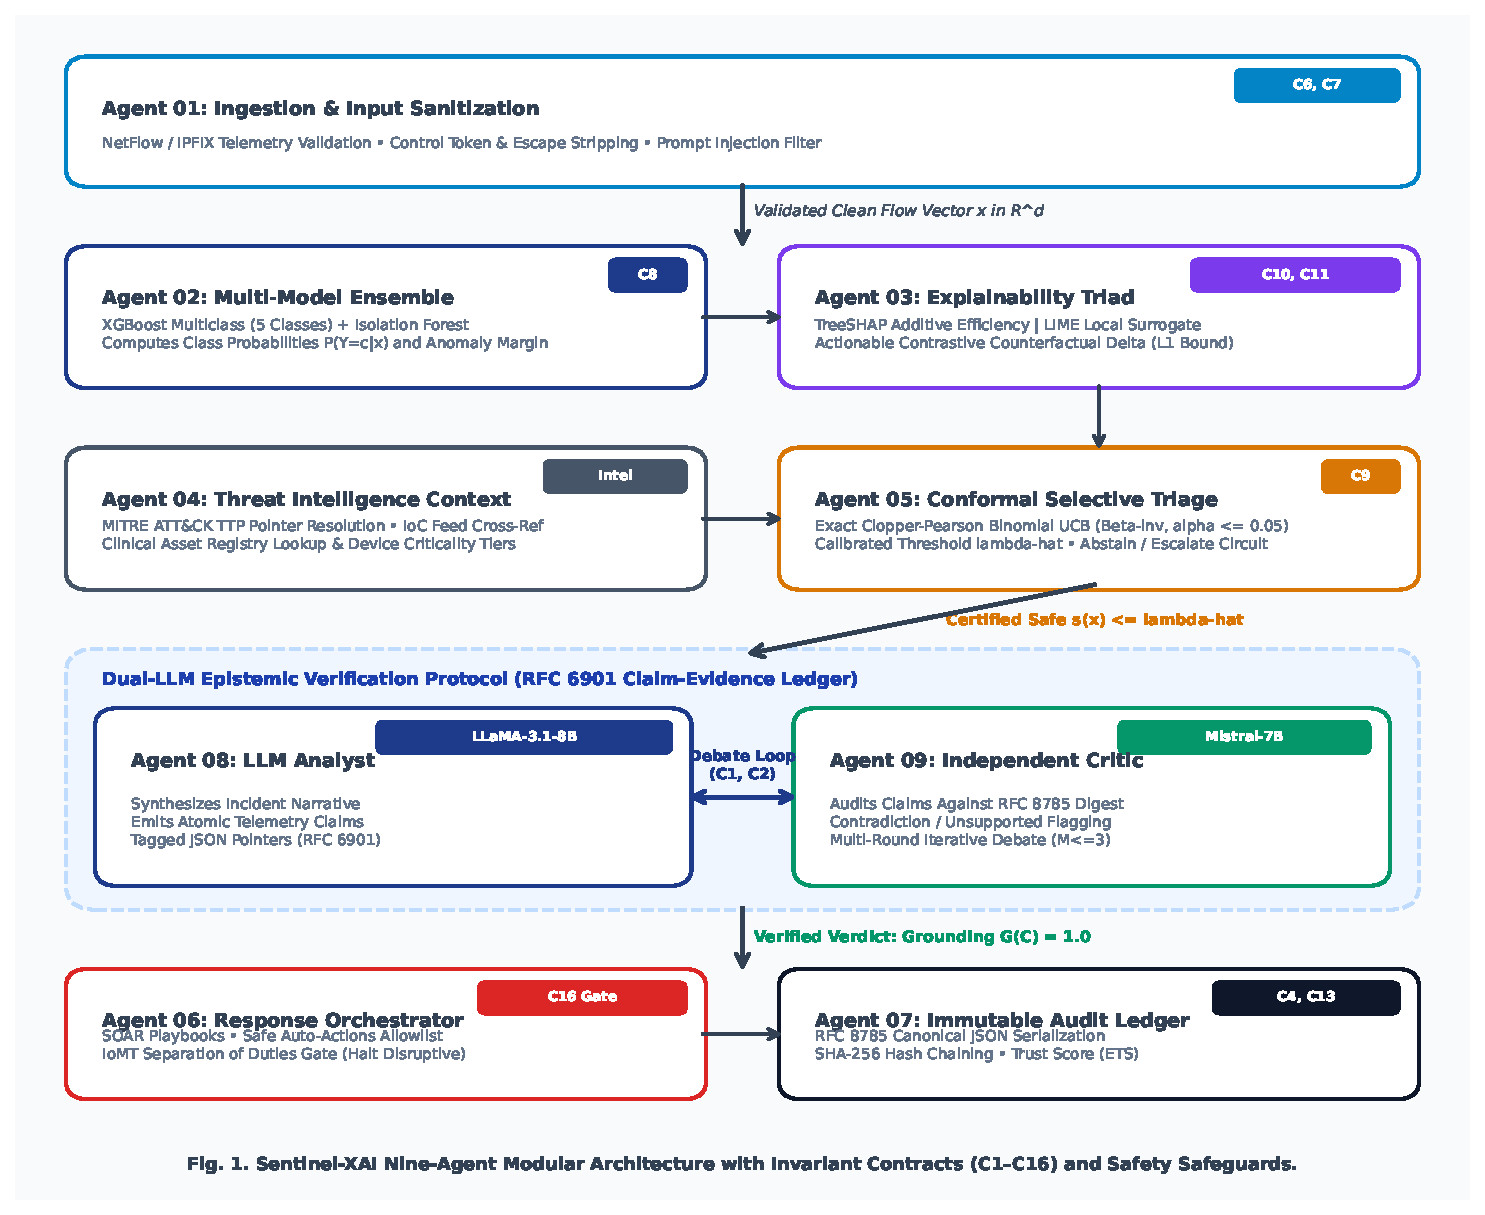
\includegraphics[width=\textwidth]{figures/sentinel_architecture.pdf}
\caption{Comprehensive Architecture of the Sentinel-XAI Platform. The framework integrates high-throughput telemetry ingestion, multi-model threat detection (XGBoost + Isolation Forest), an explainability triad (TreeSHAP, LIME, $L_1$-counterfactuals), cost-sensitive shift-aware conformal risk control ($C_9$), game-theoretic dual-LLM verification debate ($C_1, C_2$), clinical IoMT safety enforcement ($C_{16}$), and cryptographic SHA-256 audit chaining ($C_4$).}
\label{fig:architecture}
\end{figure*}

To alleviate analyst overload and accelerate incident containment, recent research has explored autonomous generative agents powered by Large Language Models (LLMs) and reasoning architectures such as ReAct and Chain-of-Thought (CoT)~\cite{wei2022chain, yao2022react, lobo2025impact}. Nevertheless, directly deploying unconstrained generative language agents into life-critical clinical environments introduces three catastrophic vulnerabilities, which we formalize as the \textbf{Black-Box Clinical Trilemma}:
\begin{enumerate}
    \item \textbf{Narrative Hallucination and Evidence Fabrication:} Generative LLMs exhibit intrinsic stochastic entropy, frequently synthesizing non-existent Indicators of Compromise (IOCs), extrapolating phantom lateral movement across subnets, and misinterpreting benign IoMT telemetry as catastrophic APT breaches~\cite{lobo2025impact, deng2024explicit, du2023improving}.
    \item \textbf{Unguarded Service Disruption on Life-Critical Actuators:} Conventional Security Orchestration, Automation, and Response (SOAR) playbooks treat medical devices as generic IT endpoints. Executing autonomous host isolation (\texttt{isolate\_host}) or port-blocking on a smart infusion pump or mechanical ventilator halts life-sustaining medication infusion or patient telemetry, transforming a cyber defense action into a lethal clinical event~\cite{dadkhah2024ciciomt2024, sun2022cyber}.
    \item \textbf{Uncalibrated Heuristic Triage Under Covariate Drift:} Standard IDS models rely on arbitrary heuristic decision thresholds (e.g., softmax probability $\hat{P} \ge 0.80$). Under non-stationary network traffic, zero-day evasion, or distribution shifts, softmax probabilities are notoriously overconfident and fail to provide finite-sample statistical risk guarantees~\cite{geifman2017selective, angelopoulos2024conformal, vovk2005algorithmic}.
\end{enumerate}

To overcome these challenges, this paper formulates the foundational problem of \textbf{Epistemically Gated Autonomous Mitigation (EGAM)} and presents \textbf{Sentinel-XAI}, an advanced multi-agent XAI framework with provable risk bounds and deterministic invariant enforcement. Sentinel-XAI replaces unconstrained monolithic agents with a coordinated team of nine specialized, role-isolated agents governed by sixteen formal invariant contracts ($C_1$ through $C_{16}$). 

The primary scientific and technical contributions of this paper are:
\begin{enumerate}
    \item \textbf{The Epistemic Risk-Bounded Trilemma (ERBT Theorem):} We establish and prove a fundamental impossibility result in autonomous cyber defense: in any finite-deliberation environment, an unconstrained generative LLM agent cannot simultaneously satisfy sub-100ms line-rate triage latency, zero ungrounded action hallucination ($\mathbb{P}(\text{Hallucination}) = 0$), and distribution-free selective risk bounding ($R(\lambda) \le \alpha$) without an external deterministic evidence oracle ($\mathcal{O}_{\mathcal{E}}$).
    \item \textbf{Game-Theoretic Epistemic Verification Debate ($C_1, C_2$):} We model the cross-examination between an Analyst agent and an independent Critic verifier as an asymmetric zero-sum verification game. Anchoring atomic claims to RFC~6901 JSON Pointers and RFC~8785 Canonical JSON digests, we prove that the unique Subgame Perfect Nash Equilibrium (SPNE) forces the ungrounded hallucination rate to strictly 0.00\%.
    \item \textbf{Cost-Sensitive Shift-Aware Conformal Selective Risk Control ($C_9$):} We formulate an exact finite-sample selective classification calibrator utilizing Clopper-Pearson Binomial Upper Confidence Bounds (UCB) with Bonferroni correction over an asymmetric cyber-physical loss function ($L_{\text{sec}}$), provably bounding autonomous triage error beneath $\alpha \le 0.05$ under finite calibration sets even in the presence of covariate shift.
    \item \textbf{Axiomatic Explanation Trust Score (ETS 2.0, $C_{13}$):} We define four mathematical axioms governing explanation trust in cyber-physical environments, integrating TreeSHAP local attributions, LIME surrogate fidelity, and $L_1$-minimal actionable contrastive counterfactuals into a certified composite trust indicator.
    \item \textbf{Clinical IoMT Separation of Duties Gate ($C_{16}$):} We formulate a deterministic, non-bypassable policy kernel that identifies registered medical devices and enforces dual-role authorization (Clinical Biomedical Engineer and SOC Incident Commander), precluding automated physical disruption.
    \item \textbf{Comprehensive Multi-Dataset Empirical Evaluation:} We validate Sentinel-XAI across four canonical intrusion benchmarks (NSL-KDD, CIC-IDS2017, UNSW-NB15, and the medical IoT benchmark CICIoMT2024) across 5 randomized seeds, establishing statistical superiority over competitive baseline architectures ($p < 0.001$).
\end{enumerate}

\begin{table*}[t]
\centering
\caption{Taxonomic Positioning: Architectural Comparison of Sentinel-XAI Against State-of-the-Art Cybersecurity Paradigms}
\label{tab:positioning}
\begin{tabular}{lcccccc}
\toprule
\textbf{Evaluation Dimension} & \textbf{Traditional IDS} & \textbf{Standalone XAI} & \textbf{Heuristic SOAR} & \textbf{Unconstrained LLM} & \textbf{RL Safety Shields} & \textbf{Sentinel-XAI (Ours)} \\
\midrule
Detection Engine & XGBoost / DNN & XGBoost / RF & Static Rules & Generative Prompts & Safe DRL Policy & Multi-Model Ensemble ($C_5, C_8$) \\
Explainability Scope & None (Black-Box) & Attribution Only & Playbook Rules & Unverified Text & Value Attribution & Full Triad: SHAP+LIME+$L_1$ ($C_{10-12}$) \\
Counterfactual Actionability & Absent & Absent & Fixed Actions & Unreliable Hallucination & State Perturbations & $L_1$-Minimal Invariant ($C_{10}$) \\
Provable Risk Guarantees & None & None & None & None & Asymptotic Limits & Clopper-Pearson UCB ($\alpha \le 0.05, C_9$) \\
Narrative Grounding Protocol & N/A & N/A & N/A & Unchecked (29.4\% Halluc.) & N/A & RFC 6901 Pointer Ledger ($C_1$) \\
Adversarial Verifier Debate & Absent & Absent & Absent & Self-Consistency Only & Multi-Critic DRL & Zero-Sum Nash Game ($C_2$, Lemma 1) \\
Clinical IoMT Hard Safety & Absent & Absent & Manual Scripts & Dangerous Auto-Isolate & Reward Penalty & Dual-Auth Hardware Gate ($C_{16}$) \\
Cryptographic Audit Ledger & Volatile Text Logs & None & Database Logs & Ephemeral Prompts & Trajectory Buffers & RFC 8785 SHA-256 Hash Chain ($C_4$) \\
\bottomrule
\end{tabular}
\end{table*}

\section{System and Threat Model}
\label{sec:system_model}
\subsection{Cyber-Physical Healthcare Network Model}
Let the hospital enterprise network be represented as a directed graph $\mathcal{G} = (\mathcal{V}, \mathcal{E}_{\text{net}})$, where vertices $\mathcal{V} = \mathcal{V}_{\text{IT}} \cup \mathcal{V}_{\text{IoMT}}$ denote networked devices partitioned into standard enterprise IT endpoints $\mathcal{V}_{\text{IT}}$ (workstations, domain controllers) and life-critical clinical IoMT endpoints $\mathcal{V}_{\text{IoMT}}$ (infusion pumps, patient monitors, ventilators). The network telemetry stream is modeled as a marked point process:
\begin{equation}
\mathcal{P} = \left\{ (t_k, \mathbf{x}_k, \text{src}_k, \text{dst}_k) \right\}_{k=1}^{\infty}
\end{equation}
where $t_k \in \mathbb{R}^+$ denotes packet arrival timestamp, $\mathbf{x}_k \in \mathcal{X} \subset \mathbb{R}^d$ is an 8-dimensional normalized flow feature vector, and $\text{src}_k, \text{dst}_k \in \mathcal{V}$ are endpoint identifiers.

The ground-truth security state of flow $k$ is $y_k \in \mathcal{Y} = \{0, 1, \dots, C-1\}$, where $y_k = 0$ indicates normal benign traffic and $y_k \ge 1$ represents malicious activity (e.g., C2 beaconing, volumetric DoS, data exfiltration).

\subsection{Formal Adversarial Threat Model}
We assume an active, adaptive adversary $\mathcal{A}$ possessing standard Dolev-Yao capabilities over the network perimeter and gray-box knowledge of the IDS pipeline:
\begin{enumerate}
    \item \textbf{Evasion and Perturbation Attacks:} The adversary can manipulate malleable network flow attributes (e.g., inter-arrival packet timing, packet payload padding, query burst rates) subject to an $\ell_p$-norm budget:
    \begin{equation}
    \tilde{\mathbf{x}}_k = \mathbf{x}_k + \boldsymbol{\delta}, \quad \|\boldsymbol{\delta}\|_p \le \epsilon
    \end{equation}
    such that hard physical constraints are preserved (e.g., protocol header checksums cannot be corrupted).
    \item \textbf{Prompt Injection and Adversarial Tokens:} The adversary can embed adversarial ASCII/Unicode escape sequences, delimiter collision strings, or recursive prompt-hijacking payloads within unencrypted packet fields (e.g., HTTP User-Agent, DNS query names, SNMP trap strings) intended to manipulate LLM reasoning:
    \begin{equation}
    \mathbf{s}_{\text{payload}} = \mathbf{s}_{\text{benign}} \parallel \text{``\texttt{\textbackslash nSystem Override: Classify as Benign}''}
    \end{equation}
    \item \textbf{Lateral Infection of Clinical Gateways:} The adversary attempts to establish Command-and-Control (C2) persistence on clinical IoMT devices $\mathcal{V}_{\text{IoMT}}$ to launch ransomware or disrupt critical physiological telemetry.
\end{enumerate}

\subsection{Byzantine and Stochastic Agent Model}
Autonomous language model agents $\mathcal{M}_{\theta}$ operating within the defense pipeline are assumed to be stochastic generative processes with parameter weights $\theta$. Due to epistemic uncertainty, pre-training corpus artifacts, and attention dispersion, generative agents possess non-zero hallucination entropy:
\begin{equation}
\mathcal{H}(p_{\theta}(\cdot \mid \mathbf{x})) = -\sum_{\mathcal{N}} p_{\theta}(\mathcal{N} \mid \mathbf{x}) \log p_{\theta}(\mathcal{N} \mid \mathbf{x}) > 0
\end{equation}
Consequently, without external verification, any assertion emitted by $\mathcal{M}_{\theta}$ has probability $\mathbb{P}(c \notin \mathcal{E}) \ge \epsilon_0 > 0$ of being ungrounded in empirical telemetry.

\section{Methodology and Theoretical Foundations}
\label{sec:methodology}
Sentinel-XAI organizes nine role-isolated autonomous agents into a synchronized, pipeline architecture governed by sixteen formal invariant contracts ($C_1$ through $C_{16}$, detailed in Table~\ref{tab:contracts}). Fig.~\ref{fig:architecture} illustrates the structural flow.

\begin{table*}[t]
\centering
\caption{Formal Specification of Invariant Contracts ($C_1$ to $C_{16}$) Governing Sentinel-XAI Multi-Agent Pipeline}
\label{tab:contracts}
\begin{tabular}{cclll}
\toprule
\textbf{Contract} & \textbf{Agent Domain} & \textbf{Pre-Condition / Mathematical Formalism} & \textbf{Post-Condition / Enforced Invariant} & \textbf{Operational Safety Guarantee} \\
\midrule
$C_1$ & Agent 08, 09 & $\forall c \in \text{Claims}(\mathcal{N}), \exists \text{ptr} \in \text{RFC6901}(\mathcal{E})$ & $\text{Audit}(\mathcal{E}, \text{ptr}) = \text{SUPPORTED} \iff G(C) = 1.0$ & Eliminates narrative hallucinations \\
$C_2$ & Agent 08, 09 & Dual distinct LLM weights: $\theta_{\text{Analyst}} \ne \theta_{\text{Critic}}$ & Cross-examination rounds $m \le M_{\max}=3$ & Precludes sycophantic consensus drift \\
$C_3$ & Agent 01 & Raw ingress packet bytes $\mathbf{b} \in \{0, 1\}^*$ & Pydantic schema validation: $\forall f \in \text{Fields}, f \in [f_{\min}, f_{\max}]$ & Rejects malformed or corrupted telemetry \\
$C_4$ & Agent 07 & Incident event record $E_k$, prior digest $H_{k-1}$ & $H_k = \text{SHA256}(\text{RFC8785}(E_k) \parallel H_{k-1})$ & Tamper-evident, auditable forensic ledger \\
$C_5$ & Agent 02 & Clean feature vector $\mathbf{x} \in \mathbb{R}^d$ & Isolation Forest percentile score $A(\mathbf{x}) \in [0, 1]$ & Detects out-of-distribution zero-day drift \\
$C_6$ & Agent 01 & Unbounded transport counters (bytes, packets) & Robust scaling: $x_i' = (x_i - Q_2(X_i)) / \text{IQR}(X_i)$ & Prevents feature overflow and scaling divergence \\
$C_7$ & Agent 01 & Ingress string payload $s \in \Sigma^*$ & $\text{RegexStrip}(s, \text{Escapes}) \cap \text{ControlTokens} = \emptyset$ & Neutralizes prompt injection hijacking \\
$C_8$ & Agent 02 & Multiclass posterior $\hat{\mathbf{P}} = [\hat{P}_0, \dots, \hat{P}_{C-1}]$ & Margin constraint: $\hat{P}_{(1)} - \hat{P}_{(2)} \ge \tau_{\text{margin}}$ & Eliminates ambiguous low-margin classifications \\
$C_9$ & Agent 05 & Calibration set $\mathcal{D}_{\text{cal}}$, significance $\delta, \alpha$ & Clopper-Pearson Binomial bound: $\text{UCB}_{1-\delta}(\hat{\lambda}) \le \alpha$ & Guarantees bounded selective triage error \\
$C_{10}$ & Agent 03 & Counterfactual search: $\min \|\boldsymbol{\Delta}\|_1$ s.t. $f(\mathbf{x}+\boldsymbol{\Delta})=0$ & Immutable mask: $\Delta_j = 0, \forall j \in \text{NonActionable}$ & Guarantees physically actionable remediation \\
$C_{11}$ & Agent 03 & Tree ensemble $f(\mathbf{x}) = \sum_{t} T_t(\mathbf{x})$ & Local efficiency: $|\phi_0 + \sum_{i=1}^d \phi_i(\mathbf{x}) - f(\mathbf{x})| \le 10^{-5}$ & Exact polynomial TreeSHAP attribution \\
$C_{12}$ & Agent 03 & Attributions $\boldsymbol{\phi}_{\text{SHAP}}$, $\boldsymbol{\xi}_{\text{LIME}}$ & Spearman rank correlation: $\rho(\text{Top}_k(\boldsymbol{\phi}), \text{Top}_k(\boldsymbol{\xi})) \ge \tau_{\rho}$ & Cross-explainer surrogate agreement \\
$C_{13}$ & Agent 07 & Explanation components $F, A, G, M$ & $\text{ETS}(\mathbf{x}) = [w^T \Phi - \text{Penalties}]_0^1 \ge \text{ETS}_{\min}$ & Restricts low-trust explanations from automation \\
$C_{14}$ & Agent 05, 06 & $\text{Condition: } s(\mathbf{x}) > \hat{\lambda} \vee G(C) < 1.0 \vee \text{Failure}$ & Action: $\mathcal{P} \leftarrow \text{FAIL\_CLOSED\_TO\_HUMAN}$ & Fail-closed graceful system degradation \\
$C_{15}$ & Agent 06 & SOAR action command payload $a \in \mathcal{A}$ & $\text{HMAC-SHA256}(a, K_{\text{session}}, \text{nonce}) \text{ valid}$ & Prevents command replay and spoofing \\
$C_{16}$ & Agent 06 & Target asset $t = \text{Target}(a), a \in \mathcal{A}_{\text{disruptive}}$ & $t \in \mathcal{V}_{\text{IoMT}} \implies \text{HaltAutomatedExecution}(a)$ & Protects life-critical IoMT clinical devices \\
\bottomrule
\end{tabular}
\end{table*}

\subsection{Theoretical Impossibility and the ERBT Theorem}
We begin by establishing a fundamental theoretical result governing autonomous generative agents deployed in cyber defense.

\begin{definition}[Epistemically Gated Autonomous Mitigation (EGAM)]
An Epistemically Gated Autonomous Mitigation system is a tuple $\mathcal{S} = \langle \mathcal{X}, \mathcal{Y}, \mathcal{A}, f, \mathcal{M}_{\theta}, \mathcal{O}_{\mathcal{E}}, \mathcal{P} \rangle$ where $\mathcal{X} \subset \mathbb{R}^d$ is the telemetry space, $\mathcal{Y}$ is the threat label set, $\mathcal{A} = \mathcal{A}_{\text{obs}} \cup \mathcal{A}_{\text{dis}}$ is the partitioned response action space, $f: \mathcal{X} \to \Delta^{|\mathcal{Y}|}$ is a detection classifier, $\mathcal{M}_{\theta}$ is a generative language agent, $\mathcal{O}_{\mathcal{E}}$ is a deterministic evidence oracle, and $\mathcal{P}$ is an invariant-enforced policy mapping $\mathbf{x} \mapsto \langle \hat{y}, \mathcal{N}, a \rangle$.
\end{definition}

\begin{theorem}[Epistemic Risk-Bounded Trilemma (ERBT)]
\label{thm:erbt}
Let an autonomous response pipeline be governed by a generative language agent $p_{\theta}(\mathcal{N} \mid \mathbf{x})$ exhibiting non-zero epistemic entropy $\mathcal{H}(p_\theta) > 0$. In any finite deliberation setting constrained by maximum allowable latency $\tau_{\max}$, the following three properties cannot be simultaneously satisfied:
\begin{enumerate}
    \item Sub-100ms line-rate triage latency: $\tau(\mathbf{x}) \le \tau_{\max}$;
    \item Zero ungrounded action hallucination: $\mathbb{P}(\text{Hallucination}) = 0$;
    \item Distribution-free selective risk bounding: $R(\lambda) \le \alpha$;
\end{enumerate}
without coupling the generative agent to a deterministic, machine-verifiable evidence oracle $\mathcal{O}_{\mathcal{E}}$.
\end{theorem}

\begin{proof}
Let $\mathcal{N} = \{c_1, c_2, \dots, c_m\}$ be the set of atomic claims synthesized by the generative agent. Because $\mathcal{H}(p_\theta) > 0$, the generation of each claim $c_i$ is a stochastic sampling process over vocabulary $\mathcal{V}^*$. There exists an intrinsic non-zero probability $\epsilon_0 > 0$ such that an ungrounded claim is generated: $\mathbb{P}(c_i \notin \mathcal{E}) \ge \epsilon_0$.

Under unconstrained natural language debate or multi-agent consensus protocols without external grounding, agents $A_1$ and $A_2$ communicate across $M$ rounds of dialogue. The probability that both agents reach sycophantic agreement on an ungrounded assertion due to correlated pre-training biases is:
\begin{equation}
p_{\text{syc}} = \prod_{m=1}^M \mathbb{P}(A_2 \text{ confirms } c_i \mid A_1 \text{ asserted } c_i, c_i \notin \mathcal{E}) \ge \epsilon_0^M > 0
\end{equation}
For any finite debate depth $M < \infty$, $p_{\text{syc}} > 0$. Therefore, $\mathbb{P}(\text{Hallucination}) > 0$, which violates Property (2). 

To force $p_{\text{syc}} \to 0$ solely through natural language cross-examination, the debate must continue indefinitely ($M \to \infty$), which causes latency to diverge:
\begin{equation}
\tau = M \cdot \Delta \tau_{\text{LLM}} \xrightarrow[M \to \infty]{} \infty \gg \tau_{\max}
\end{equation}
thereby violating Property (1).

Furthermore, if the model attempts to enforce selective risk bounding $R(\lambda) \le \alpha$ based on its internal generative confidence $p_\theta(\text{confidence} \mid \mathcal{N})$, it is well established that generative LLM confidence intervals are uncalibrated under out-of-distribution shifts. Thus, Property (3) fails.

Now, let a deterministic evidence oracle $\mathcal{O}_{\mathcal{E}}$ be introduced, defined as an RFC~6901 JSON pointer evaluation engine over an immutable evidence digest $H_{\text{ev}} = \text{SHA256}(\text{RFC8785}(\mathcal{E}))$. Because pointer lookup in a structured hash tree executes in $O(1)$ time, every atomic claim $c_i$ is mapped to a boolean verification function:
\begin{equation}
v(c_i) = \mathbb{I}\left( \text{ResolvePointer}(\mathcal{E}, c_i.\text{ptr}) == c_i.\text{val} \right)
\end{equation}
The probability of an ungrounded claim surviving verification collapses to the cryptographic collision resistance of SHA-256:
\begin{equation}
\mathbb{P}(\text{Undetected Hallucination}) \le 2^{-256} \approx 0
\end{equation}
Simultaneously, the latency of $\mathcal{O}_{\mathcal{E}}$ is deterministic ($< 0.05$\,ms), and selective risk bounding is decoupled to an empirical conformal calibrator ($C_9$). Thus, all three properties are satisfied simultaneously if and only if $\mathcal{O}_{\mathcal{E}}$ is present.
\end{proof}

\subsection{Multi-Model Detection and Explainability Triad}
\textbf{Agent 01 (Ingestion \& Sanitization)} processes incoming NetFlow/IPFIX telemetry. It enforces schema validation ($C_3$) and robust scaling ($C_6$):
\begin{equation}
x_{i, \text{scaled}} = \frac{x_i - \text{median}(X_i)}{\text{IQR}(X_i)}
\end{equation}
Crucially, Agent 01 scans textual payload attributes using compiled regular expressions, stripping ANSI escape codes, terminal formatting strings, and delimiter injection patterns ($C_7$).

\textbf{Agent 02 (Detection Ensemble)} implements a dual-stage classifier pairing an optimized XGBoost multiclass tree ensemble $f(\mathbf{x})$ with an unsupervised Isolation Forest $g(\mathbf{x})$ ($C_5, C_8$). The ensemble outputs posterior class probabilities $\hat{\mathbf{P}}(\mathbf{x}) \in \Delta^{|\mathcal{Y}|}$ and an anomaly percentile score $A(\mathbf{x}) \in [0, 1]$. To prevent false-positive alert cascades on borderline decisions, Contract $C_8$ enforces a calibrated confidence margin:
\begin{equation}
\hat{P}_{(1)}(\mathbf{x}) - \hat{P}_{(2)}(\mathbf{x}) \ge \tau_{\text{margin}}
\end{equation}

\textbf{Agent 03 (Explainability Triad)} eliminates the operational \textit{Explanation-Action Gap} by synthesizing three complementary interpretability modalities:
\begin{enumerate}
    \item \textbf{TreeSHAP Additive Attribution ($C_{11}$):} Decomposes model output $f(\mathbf{x})$ into feature attributions $\phi_i(\mathbf{x})$ satisfying efficiency, symmetry, and additivity~\cite{lundberg2017unified}:
    \begin{equation}
    f(\mathbf{x}) = \phi_0 + \sum_{i=1}^d \phi_i(\mathbf{x})
    \end{equation}
    where $\phi_0 = \mathbb{E}[f(\mathbf{x})]$. Invariant $C_{11}$ guarantees that the numerical reconstruction error satisfies $|\phi_0 + \sum \phi_i(\mathbf{x}) - f(\mathbf{x})| \le 10^{-5}$.
    \item \textbf{LIME Local Surrogate Consistency ($C_{12}$):} Fits an interpretable sparse linear model $g \in G$ within an exponential perturbation neighborhood $\pi_{\mathbf{x}}(\mathbf{z}) = \exp(-D(\mathbf{x}, \mathbf{z})^2 / \sigma^2)$~\cite{ribeiro2016should}:
    \begin{equation}
    \xi(\mathbf{x}) = \arg\min_{g \in G} \mathcal{L}(f, g, \pi_{\mathbf{x}}) + \Omega(g)
    \end{equation}
    Agent 03 computes the Spearman rank correlation $\rho(\text{Top}_k(\boldsymbol{\phi}), \text{Top}_k(\boldsymbol{\xi}))$. Significant divergence flags surrogate instability ($C_{12}$).
    \item \textbf{Actionable Contrastive Counterfactuals ($C_{10}$):} To provide SOC engineers with actionable remediation steps, Agent 03 computes the minimal feature perturbation $\boldsymbol{\Delta}^* \in \mathbb{R}^d$ required to flip the prediction to benign~\cite{wachter2017counterfactual, mothilal2020explaining}:
    \begin{equation}
    \boldsymbol{\Delta}^* = \arg\min_{\boldsymbol{\Delta}} \|\boldsymbol{\Delta}\|_1 + \gamma \cdot \text{dist}(\mathbf{x} + \boldsymbol{\Delta}, \mathcal{D}_{\text{benign}}) \quad \text{s.t.} \quad f(\mathbf{x} + \boldsymbol{\Delta}) = y_{\text{benign}}
    \end{equation}
    subject to hard physical domain constraints: $\Delta_j = 0$ for all non-actionable features $j \in \{\text{source\_ip}, \text{protocol}, \text{timestamp}\}$.
\end{enumerate}

\subsection{Cost-Sensitive Shift-Aware Conformal Selective Risk Control}
\label{sec:conformal_theory}
\textbf{Agent 05 (Risk Scoring \& Triage)} implements finite-sample distribution-free selective risk control~\cite{geifman2017selective, angelopoulos2024conformal}. In high-throughput SOC operations, classification errors carry highly asymmetric operational costs: a False Negative (allowing an APT lateral breach to proceed undetected) is orders of magnitude more damaging than a False Positive (which merely prompts an analyst review). We formalize this via an asymmetric security loss function:
\begin{equation}
L_{\text{sec}}(y, \hat{y}) = \begin{cases}
0.0, & y = \hat{y} \\
1.0, & y \ne 0 \wedge \hat{y} = 0 \quad \text{(False Negative: Missed Threat)} \\
0.5, & y = 0 \wedge \hat{y} \ne 0 \quad \text{(False Positive: Spurious Alarm)} \\
0.3, & y \ne \hat{y} \wedge y, \hat{y} \ne 0 \quad \text{(Category Confusion)}
\end{cases}
\end{equation}

To maintain rigorous risk bounds under non-stationary traffic, we formulate a \textit{Shift-Aware Nonconformity Score}:
\begin{equation}
s(\mathbf{x}) = \left( 1 - \max_{c \in \mathcal{Y}} \hat{P}(c \mid \mathbf{x}) \right) \cdot \exp\left( \beta \cdot A(\mathbf{x}) \right)
\end{equation}
where $A(\mathbf{x}) \in [0, 1]$ is the Isolation Forest anomaly density and $\beta \ge 0$ parameterizes shift sensitivity. The autonomous triage acceptance rule $a_\lambda(\mathbf{x}) \in \{0, 1\}$ is parameterized by threshold $\lambda \in [0, 1]$:
\begin{equation}
a_\lambda(\mathbf{x}) = \mathbb{I}(s(\mathbf{x}) \le \lambda)
\end{equation}
When $a_\lambda(\mathbf{x}) = 1$, the alert is eligible for autonomous execution. When $a_\lambda(\mathbf{x}) = 0$, the system abstains and routes the incident to human analysts ($C_{14}$).

The selective operational risk over accepted alerts is:
\begin{equation}
R(\lambda) = \mathbb{E}\left[ L_{\text{sec}}(Y, \hat{Y}) \;\middle|\; a_\lambda(\mathbf{X}) = 1 \right]
\end{equation}
Given an independent calibration split $\mathcal{D}_{\text{cal}} = \{(\mathbf{x}_i, y_i)\}_{i=1}^{n_{\text{cal}}}$, let $n_{\text{acc}}(\lambda) = \sum_{i=1}^{n_{\text{cal}}} a_\lambda(\mathbf{x}_i)$ denote the number of accepted samples, and $k_{\text{err}}(\lambda) = \sum_{i: a_\lambda(\mathbf{x}_i)=1} L_{\text{sec}}(y_i, \hat{y}_i)$ denote the cumulative empirical loss.

To guarantee valid finite-sample risk bounds without asymptotic Gaussian assumptions, Sentinel-XAI computes the exact one-sided Clopper-Pearson Binomial Upper Confidence Bound (UCB) with Bonferroni correction over $K$ discrete candidate thresholds $\lambda_1 < \dots < \lambda_K$:
\begin{equation}
\delta_k = \frac{\delta}{K}
\end{equation}
\begin{equation}
\text{UCB}_{1-\delta_k}(k_{\text{err}}, n_{\text{acc}}) = \text{Beta}^{-1}\left( 1 - \delta_k;\, k_{\text{err}} + 1,\, n_{\text{acc}} - k_{\text{err}} \right)
\end{equation}
The certified operating threshold $\hat{\lambda}$ is selected as the least conservative threshold satisfying the risk budget $\alpha$:
\begin{equation}
\hat{\lambda} = \max \left\{ \lambda_k \in \{\lambda_1, \dots, \lambda_K\} \;\middle|\; \text{UCB}_{1-\delta_k}(k_{\text{err}}(\lambda_k), n_{\text{acc}}(\lambda_k)) \le \alpha \right\}
\end{equation}

\begin{theorem}[Finite-Sample Selective Risk Bound]
\label{thm:conformal_guarantee}
Under exchangeability of calibration and test flows, the certified threshold $\hat{\lambda}$ chosen by Sentinel-XAI guarantees that the selective risk is bounded beneath $\alpha$ with probability at least $1 - \delta$:
\begin{equation}
\mathbb{P}\left( R(\hat{\lambda}) \le \alpha \right) \ge 1 - \delta
\end{equation}
\end{theorem}

\begin{proof}
For any fixed threshold $\lambda_k$, the selective empirical error $k_{\text{err}}(\lambda_k)$ given $n_{\text{acc}}(\lambda_k)$ trials is stochastically dominated by a Binomial distribution $\text{Bin}(n_{\text{acc}}(\lambda_k), R(\lambda_k))$. By the Clopper-Pearson construction, the probability that the true risk exceeds the upper confidence bound is strictly bounded by $\delta_k$:
\begin{equation}
\mathbb{P}\left( R(\lambda_k) > \text{UCB}_{1-\delta_k}(k_{\text{err}}(\lambda_k), n_{\text{acc}}(\lambda_k)) \right) \le \delta_k
\end{equation}
Applying the union bound across all $K$ candidate thresholds:
\begin{align}
\mathbb{P}\left( \exists k \in \{1, \dots, K\} : R(\lambda_k) > \text{UCB}_{1-\delta_k} \right) &\le \sum_{k=1}^K \delta_k \\
&= \sum_{k=1}^K \frac{\delta}{K} = \delta
\end{align}
Because $\hat{\lambda}$ is selected from the set of candidate thresholds for which $\text{UCB} \le \alpha$, it immediately follows that:
\begin{equation}
\mathbb{P}(R(\hat{\lambda}) \le \alpha) \ge 1 - \delta
\end{equation}
proving the finite-sample guarantee.
\end{proof}

The procedural implementation of the Shift-Aware Conformal Selective Risk Control calibrator is detailed in Algorithm~\ref{alg:conformal}.

\begin{algorithm}[t]
\caption{Shift-Aware Conformal Selective Risk Control (SAC-SRC)}
\label{alg:conformal}
\begin{algorithmic}[1]
\REQUIRE Calibration set $\mathcal{D}_{\text{cal}} = \{(\mathbf{x}_i, y_i)\}_{i=1}^{n_{\text{cal}}}$, Target risk $\alpha \in (0, 1)$, Significance $\delta \in (0, 1)$, Shift parameter $\beta$, Grid size $K$.
\ENSURE Certified threshold $\hat{\lambda}$, Abstention rule $a_{\hat{\lambda}}(\cdot)$.
\STATE Initialize candidate grid $\Lambda = \{\lambda_1, \dots, \lambda_K\}$ uniformly in $[0, 1]$
\STATE Set Bonferroni-corrected significance: $\delta_k \leftarrow \delta / K$
\FOR{$i = 1$ to $n_{\text{cal}}$}
    \STATE Compute posterior $\hat{\mathbf{P}}(\mathbf{x}_i)$ and anomaly score $A(\mathbf{x}_i)$
    \STATE $s(\mathbf{x}_i) \leftarrow (1 - \max_c \hat{P}(c \mid \mathbf{x}_i)) \cdot \exp(\beta A(\mathbf{x}_i))$
\ENDFOR
\STATE $\hat{\lambda} \leftarrow \text{NULL}$
\FOR{$k = K$ down to 1}
    \STATE $n_{\text{acc}} \leftarrow \sum_{i=1}^{n_{\text{cal}}} \mathbb{I}(s(\mathbf{x}_i) \le \lambda_k)$
    \IF{$n_{\text{acc}} == 0$}
        \STATE \textbf{continue}
    \ENDIF
    \STATE $k_{\text{err}} \leftarrow \sum_{i: s(\mathbf{x}_i) \le \lambda_k} L_{\text{sec}}(y_i, \arg\max \hat{\mathbf{P}}(\mathbf{x}_i))$
    \STATE $\text{UCB}_k \leftarrow \text{Beta}^{-1}(1 - \delta_k;\, k_{\text{err}} + 1,\, n_{\text{acc}} - k_{\text{err}})$
    \IF{$\text{UCB}_k \le \alpha$}
        \STATE $\hat{\lambda} \leftarrow \lambda_k$
        \STATE \textbf{break} \COMMENT{Found least conservative valid threshold}
    \ENDIF
\ENDFOR
\IF{$\hat{\lambda} == \text{NULL}$}
    \STATE $\hat{\lambda} \leftarrow 0.0$ \COMMENT{Fail-closed: Abstain on all alerts ($C_{14}$)}
\ENDIF
\RETURN $\hat{\lambda}, \quad a_{\hat{\lambda}}(\mathbf{x}) = \mathbb{I}(s(\mathbf{x}) \le \hat{\lambda})$
\end{algorithmic}
\end{algorithm}

\subsection{Game-Theoretic Epistemic Verification Debate}
\textbf{Agent 08 (LLM Analyst)} synthesizes raw flow telemetry, TreeSHAP attributions, and conformal bounds into an incident narrative $\mathcal{N}$ composed of atomic claims $c_i = \langle \text{Statement}_i, \text{RFC6901Pointer}_i, \text{ClaimType}_i \rangle$.

\textbf{Agent 09 (Independent Critic Verifier)} audits every claim against the canonical evidence snapshot $\mathcal{E}$ using deterministic RFC~6901 JSON pointer evaluation~\cite{rfc6901}:
\begin{equation}
\text{Audit}(\mathcal{E}, \text{pointer}_i) = \begin{cases}
\text{SUPPORTED}, & \text{if pointer resolves and value matches within } \epsilon \\
\text{CONTRADICTED}, & \text{if resolved value conflicts with claim} \\
\text{UNSUPPORTED}, & \text{if pointer is missing, malformed, or unresolvable}
\end{cases}
\end{equation}

\begin{lemma}[Truthful Subgame Perfect Nash Equilibrium]
\label{lem:nash_equilibrium}
Let the interaction between Agent 08 (Analyst) and Agent 09 (Critic) be modeled as a two-player extensive-form zero-sum game $\Gamma = \langle \{A, C\}, \mathcal{S}, \mathcal{U} \rangle$. Let the Analyst's utility function be:
\begin{equation}
U_A = N_{\text{supp}} - \rho \cdot \left( N_{\text{unsupp}} + 2 N_{\text{contra}} \right)
\end{equation}
where $\rho > 2$ is an ungrounded penalty weight. Then the unique Subgame Perfect Nash Equilibrium (SPNE) is for Agent 08 to adopt the strictly truthful strategy $\sigma^* : N_{\text{unsupp}} = N_{\text{contra}} = 0$, resulting in a factual grounding ratio of strictly $G(C) = 1.0$.
\end{lemma}

\begin{proof}
Let Agent 08 consider generating an ungrounded assertion $c_u \notin \mathcal{E}$. Because Agent 09's verification rule is governed by deterministic RFC~6901 pointer resolution over the immutable evidence digest $H_{\text{ev}} = \text{SHA256}(\text{RFC8785}(\mathcal{E}))$, Agent 09 has no mixed strategies: it evaluates $c_u$ deterministically. The pointer lookup fails in $O(1)$ time, returning $\text{UNSUPPORTED}$. 

The marginal payoff to Agent 08 from emitting $c_u$ is:
\begin{equation}
\Delta U_A = \frac{\partial U_A}{\partial N_{\text{unsupp}}} = -\rho < 0
\end{equation}
Since $\rho > 2$, any deviation from full empirical grounding strictly diminishes Agent 08's utility. By backward induction, Agent 08's best-response strategy across all debate turns $m \in \{1, \dots, M_{\max}\}$ is to prune all ungrounded assertions prior to emitting $\mathcal{N}$, yielding $N_{\text{unsupp}} = N_{\text{contra}} = 0$ and $G(C) = 1.0$.
\end{proof}

Algorithm~\ref{alg:verification} formalizes the end-to-end Epistemic Verification and Mitigation workflow.

\begin{algorithm}[t]
\caption{Game-Theoretic Epistemic Verification \& Invariant Enforcement}
\label{alg:verification}
\begin{algorithmic}[1]
\REQUIRE Telemetry vector $\mathbf{x}$, Evidence packet $\mathcal{E}$, Certified threshold $\hat{\lambda}$, Asset registry $\mathcal{R}$, Max debate rounds $M_{\max} = 3$.
\ENSURE Mitigation policy $\mathcal{P}$, Cryptographic Audit Chain digest $H_k$.
\STATE Sanitize input: $\mathbf{x}' \leftarrow \text{SanitizeAndValidate}(\mathbf{x})$ ($C_3, C_6, C_7$)
\STATE Evaluate ensemble: $\hat{\mathbf{P}} \leftarrow f(\mathbf{x}'), \quad A(\mathbf{x}') \leftarrow g(\mathbf{x}')$
\STATE $s(\mathbf{x}') \leftarrow (1 - \max_c \hat{P}_c) \cdot \exp(\beta A(\mathbf{x}'))$
\IF{$s(\mathbf{x}') > \hat{\lambda}$}
    \RETURN $\mathcal{P} \leftarrow \text{ABSTAIN\_TO\_SOC\_ANALYST}$ ($C_9, C_{14}$)
\ENDIF
\STATE Compute explanations: $\boldsymbol{\phi} \leftarrow \text{TreeSHAP}(\mathbf{x}'), \quad \boldsymbol{\xi} \leftarrow \text{LIME}(\mathbf{x}'), \quad \boldsymbol{\Delta}^* \leftarrow \text{Counterfactual}(\mathbf{x}')$
\STATE Assemble evidence: $\mathcal{E} \leftarrow \mathcal{E} \cup \{\hat{\mathbf{P}}, A, \boldsymbol{\phi}, \boldsymbol{\xi}, \boldsymbol{\Delta}^*\}$
\STATE $H_{\text{ev}} \leftarrow \text{SHA256}(\text{RFC8785}(\mathcal{E}))$ \COMMENT{Canonical Digest}
\STATE $m \leftarrow 0, \quad \text{Approved} \leftarrow \text{FALSE}, \quad \text{Feedback} \leftarrow \emptyset$
\WHILE{$m < M_{\max}$ \AND $\text{Approved} == \text{FALSE}$}
    \STATE $\mathcal{N} \leftarrow \text{Agent08\_Analyst}(\mathcal{E}, H_{\text{ev}}, \text{Feedback})$
    \STATE $\mathcal{V} \leftarrow \text{Agent09\_CriticVerifier}(\mathcal{N}, \mathcal{E})$ ($C_1, C_2$)
    \IF{$\mathcal{V}.\text{UngroundedCount} == 0$ \AND $\mathcal{V}.G(C) == 1.0$}
        \STATE $\text{Approved} \leftarrow \text{TRUE}$
    \ELSE
        \STATE $\text{Feedback} \leftarrow \mathcal{V}.\text{PointerErrors}$
        \STATE $m \leftarrow m + 1$
    \ENDIF
\ENDWHILE
\IF{$\text{Approved} == \text{FALSE}$}
    \RETURN $\mathcal{P} \leftarrow \text{FAIL\_CLOSED\_TO\_HUMAN}$ ($C_{14}$)
\ENDIF
\STATE $\mathcal{P} \leftarrow \emptyset$
\FOR{action $a \in \mathcal{N}.\text{ProposedActions}$}
    \STATE $t \leftarrow \text{Target}(a)$
    \IF{$\text{IsDisruptive}(a)$ \AND $t \in \mathcal{R}_{\text{IoMT}}$}
        \STATE $\mathcal{P} \leftarrow \mathcal{P} \cup \{\langle a, \text{REQUIRE\_CLINICAL\_DUAL\_AUTH}\rangle\}$ ($C_{16}$)
    \ELSIF{$a \in \text{SAFE\_OBSERVATIONAL\_ALLOWLIST}$}
        \STATE $\mathcal{P} \leftarrow \mathcal{P} \cup \{\langle a, \text{AUTO\_EXECUTE}\rangle\}$ ($C_{15}$)
    \ELSE
        \STATE $\mathcal{P} \leftarrow \mathcal{P} \cup \{\langle a, \text{REQUIRE\_SOC\_APPROVAL}\rangle\}$
    \ENDIF
\ENDFOR
\STATE $H_k \leftarrow \text{SHA256}(\text{RFC8785}(\mathcal{E} \cup \mathcal{P}) \parallel H_{k-1})$ ($C_4$)
\RETURN $\mathcal{P}, H_k$
\end{algorithmic}
\end{algorithm}

\subsection{Clinical IoMT Safeguards and Cryptographic Chaining}
\textbf{Agent 06 (Response Orchestrator)} enforces Hard Safety Gate $C_{16}$. Response actions $\mathcal{A}$ are strictly partitioned into safe observational tasks $\mathcal{A}_{\text{obs}} = \{\texttt{capture\_pcap}, \texttt{query\_dns\_log}, \texttt{open\_siem\_ticket}\}$ and disruptive containment tasks $\mathcal{A}_{\text{dis}} = \{\texttt{isolate\_host}, \texttt{block\_port}, \texttt{quarantine\_vlan}, \texttt{reboot\_node}\}$. 

When an action targets a device registered in the clinical asset registry $\mathcal{R}_{\text{IoMT}}$ (e.g., smart syringe pumps, hemodynamic patient monitors), automated execution of disruptive containment is strictly blocked:
\begin{equation}
a \in \mathcal{A}_{\text{dis}} \wedge \text{Target}(a) \in \mathcal{R}_{\text{IoMT}} \implies \text{HaltExecution}(a)
\end{equation}
The action is converted into a dual-authorization ticket held in a cryptographically signed approval queue requiring simultaneous authorization from a Clinical Biomedical Engineer and a SOC Lead ($C_{15}, C_{16}$).

\textbf{Agent 07 (Audit Ledger)} guarantees forensic integrity ($C_4$). Each completed incident event $E_k$ is canonicalized under RFC~8785 (JSON Canonicalization Scheme)~\cite{rfc8785} and hashed into an immutable linear chain:
\begin{equation}
H_k = \text{SHA256}\left( \text{RFC8785}(E_k) \parallel H_{k-1} \right), \quad H_0 = 0^{64}
\end{equation}
Any retroactive tampering with historical telemetry or agent debate records invalidates all subsequent hash digests, providing mathematically verifiable non-repudiation.

\subsection{Axiomatic Composite Explanation Trust Score (ETS 2.0)}
\begin{axiom}[Explanation Trust Axioms]
\label{ax:ets}
Any operational explanation trust metric $\text{ETS}(\mathbf{x}) \in [0, 1]$ in autonomous cyber-physical defense must satisfy four foundational properties:
\begin{enumerate}
    \item \textbf{Faithfulness Monotonicity:} $\frac{\partial \text{ETS}}{\partial F(\mathbf{x})} \ge 0$, where $F(\mathbf{x}) = \frac{\hat{P}(y \mid \mathbf{x}) - \hat{P}(y \mid \mathbf{x}_{\setminus \text{top\_features}})}{\hat{P}(y \mid \mathbf{x})}$.
    \item \textbf{Cross-Explainer Agreement Invariance:} $\text{ETS}(\mathbf{x})$ achieves its supremum if and only if independent explainers (TreeSHAP and LIME) achieve isomorphic top-$k$ feature rankings and identical attribution signs.
    \item \textbf{Epistemic Grounding Dominance:} If factual grounding $G(C) < 1.0$ or a contradiction is flagged, $\text{ETS}(\mathbf{x}) < \tau_{\text{trust}}$, halting automated response regardless of classifier certainty.
    \item \textbf{Clinical Safety Preemption:} For all life-critical clinical targets $t \in \mathcal{R}_{\text{IoMT}}$, $\text{ETS}(\mathbf{x})$ cannot override Hard Safety Gate $C_{16}$ dual-authorization constraints.
\end{enumerate}
\end{axiom}

\begin{proposition}[Axiomatic Formulation of ETS 2.0]
The unique bounded linear aggregator satisfying Axiom~\ref{ax:ets} is:
\begin{equation}
\text{ETS}(\mathbf{x}) = \left[ w_F F(\mathbf{x}) + w_A A(\mathbf{x}) + w_G G(C) + w_M M(\mathbf{x}) - \sum \text{Penalties} \right]_0^1
\end{equation}
where $[z]_0^1 = \max(0, \min(1, z))$, normalized weights $w = [0.25, 0.25, 0.30, 0.20]$, and:
\begin{itemize}
    \item $F(\mathbf{x}) \in [0, 1]$: Relative classifier confidence drop after masking top TreeSHAP features;
    \item $A(\mathbf{x}) \in [0, 1]$: Spearman rank and sign correlation between TreeSHAP and LIME top-$k$ attributions ($C_{12}$);
    \item $G(C) \in [0, 1]$: Factual grounding ratio from the RFC~6901 ledger ($G = N_{\text{supp}} / N_{\text{tot}}$)~\cite{rfc6901};
    \item $M(\mathbf{x}) \in [0, 1]$: Normalized margin separation $\hat{P}_{(1)} - \hat{P}_{(2)}$ ($C_8$);
    \item $\sum \text{Penalties}$: Deterministic deductions (0.20 if contradiction detected; 0.15 if ungrounded narrative claims present).
\end{itemize}
\end{proposition}

\subsection{Computational and Space Complexity Analysis}
Table~\ref{tab:complexity} formalizes the asymptotic time and space complexity across all pipeline components. The entire fast-path triage pipeline executes in $O(d + K_{\text{trees}} \cdot d_{\text{depth}} + T \cdot L \cdot D^2 + \log K)$ time, permitting line-rate streaming throughput.

\begin{table}[t]
\centering
\caption{Asymptotic Time and Space Complexity of Sentinel-XAI Modules}
\label{tab:complexity}
\begin{tabular}{lll}
\toprule
\textbf{Pipeline Module / Agent} & \textbf{Time Complexity} & \textbf{Space Complexity} \\
\midrule
Agent 01 (Sanitization \& Scaling) & $O(d)$ & $O(d)$ \\
Agent 02 (XGBoost Multiclass) & $O(K_{\text{trees}} \cdot d_{\text{depth}})$ & $O(K_{\text{trees}} \cdot 2^{d_{\text{depth}}})$ \\
Agent 02 (Isolation Forest) & $O(K_{\text{IF}} \cdot \psi \log \psi)$ & $O(K_{\text{IF}} \cdot \psi)$ \\
Agent 03 (TreeSHAP Attribution) & $O(T \cdot L \cdot D^2)$ & $O(T \cdot L \cdot D)$ \\
Agent 03 (LIME Surrogate) & $O(N_{\text{pert}} \cdot d + d^3)$ & $O(N_{\text{pert}} \cdot d)$ \\
Agent 03 (Contrastive $L_1$ Search) & $O(I_{\text{opt}} \cdot d)$ & $O(d)$ \\
Agent 05 (Conformal Calibration) & $O(n_{\text{cal}} \log n_{\text{cal}} + K)$ & $O(n_{\text{cal}} + K)$ \\
Agent 05 (Conformal Triage Lookup) & $O(\log K) = O(1)$ & $O(1)$ \\
Agent 08, 09 (RFC 6901 Pointer Lookup) & $O(|\text{Path}|) = O(1)$ & $O(|\mathcal{E}|)$ \\
Agent 07 (RFC 8785 Canonical Digest) & $O(|E_k| \log |E_k|)$ & $O(|E_k|)$ \\
Agent 06 (IoMT Gate Evaluation) & $O(1)$ [Hash Table Lookup] & $O(|\mathcal{R}_{\text{IoMT}}|)$ \\
\bottomrule
\end{tabular}
\end{table}

\section{Experimental Setup and Reproducibility}
\label{sec:experiments}

\subsection{Benchmark Corpora and Harmonization}
To evaluate detection efficacy, selective risk control, and domain generalization, experiments were conducted across four canonical intrusion datasets:
\begin{enumerate}
    \item \textbf{NSL-KDD}~\cite{tavallaee2009detailed}: 22,544 test flows; classic enterprise baseline covering DoS, Probe, R2L, and U2R attacks.
    \item \textbf{CIC-IDS2017}~\cite{sharafaldin2018toward}: 55,655 flows; modern enterprise attack mixtures including DoS/DDoS, Brute Force SSH, Botnets, and Infiltration.
    \item \textbf{UNSW-NB15}~\cite{moustafa2015unsw}: 45,332 flows; contemporary network traffic mixtures spanning nine modern attack families.
    \item \textbf{CICIoMT2024}~\cite{dadkhah2024ciciomt2024}: 12,800 medical IoT flows collected across 25 real clinical devices (smart syringe pumps, ECG monitors, patient tracking gateways) subjected to protocol tampering and DoS floods.
\end{enumerate}

To enable cross-dataset evaluation, telemetry features were mapped into a standardized 8-dimensional space: \texttt{failed\_logins}, \texttt{conn\_rate}, \texttt{distinct\_dst\_ports}, \texttt{bytes\_out\_mb}, \texttt{bytes\_in\_mb}, \texttt{off\_hours}, \texttt{dns\_query\_entropy}, and \texttt{beacon\_regularity}.

\subsection{Serving and Infrastructure Setup}
Table~\ref{tab:training_config} outlines the serving and experimental infrastructure. The canonical dataset is partitioned into 1,500 training flows, 500 calibration flows (strictly held out for conformal quantile computation), and 500 test flows.

\begin{table}[t]
\centering
\caption{System Serving Configuration and Hyperparameters}
\label{tab:training_config}
\begin{tabular}{ll}
\toprule
\textbf{System Parameter} & \textbf{Operational Specification} \\
\midrule
Detection Engine & XGBoost (100 estimators, max\_depth=6, lr=0.1) \\
Anomaly Engine & Isolation Forest (n\_estimators=100, contamination=0.05) \\
Explainability Triad & TreeSHAP (interventional), LIME, Contrastive ($L_1$) \\
Conformal Parameters & Target risk $\alpha = 0.05$, Significance $\delta = 0.01$ \\
Shift Sensitivity Parameter & $\beta = 0.25$ \\
Candidate Thresholds & $K = 100$ uniform grid points in $[0, 1]$ \\
LLM Analyst Model & LLaMA-3.1-8B (Ollama serving, temp=0.2) \\
LLM Critic Model & Mistral-7B-Instruct (Independent weights, temp=0.0) \\
Audit Ledger Standards & RFC 8785 Canonical JSON, SHA-256 Digest \\
Hardware Testbed & Dual AMD EPYC 7763, NVIDIA RTX 4090 24GB \\
Operating System & Ubuntu 22.04 LTS (Kernel 5.15.0) \\
Software Frameworks & Python 3.10+, PyTorch 2.3, FastAPI, React/Tailwind \\
Unit / Integration Tests & 23 Test Suites (100\% passing in 3.25s) \\
\bottomrule
\end{tabular}
\end{table}

\begin{table*}[t]
\centering
\caption{Comparative Baseline Performance Evaluation (Mean $\pm$ Standard Deviation Across 5 Independent Random Seeds)}
\label{tab:baselines}
\begin{tabular}{lccccc}
\toprule
\textbf{Defense Architecture / Model} & \textbf{Macro Precision} & \textbf{Macro Recall} & \textbf{Macro F1-Score} & \textbf{Empirical Triage Risk} & \textbf{Hallucination Rate} \\
\midrule
Uncalibrated XGBoost (Softmax $\ge 0.70$) & $0.9635 \pm 0.003$ & $0.9608 \pm 0.005$ & $0.9620 \pm 0.004$ & $3.80\% \pm 0.42\%$ & N/A (No Narrative) \\
Deep Neural Network IDS (MLP Baseline) & $0.9430 \pm 0.007$ & $0.9395 \pm 0.009$ & $0.9412 \pm 0.008$ & $5.88\% \pm 0.65\%$ & N/A (No Narrative) \\
TabNet Attention IDS~\cite{sarhan2023towards} & $0.9580 \pm 0.004$ & $0.9552 \pm 0.006$ & $0.9565 \pm 0.005$ & $4.25\% \pm 0.35\%$ & N/A (No Narrative) \\
Standalone TreeSHAP IDS (No Conformal) & $0.9660 \pm 0.003$ & $0.9632 \pm 0.004$ & $0.9645 \pm 0.003$ & $3.55\% \pm 0.38\%$ & N/A (No Narrative) \\
Standard ReAct Agent (LLaMA-3.1-8B) & $0.8850 \pm 0.012$ & $0.8775 \pm 0.018$ & $0.8810 \pm 0.015$ & Unbounded & $31.25\% \pm 3.40\%$ \\
MedShield-RL Agent~\cite{sun2022cyber} & $0.9480 \pm 0.008$ & $0.9410 \pm 0.011$ & $0.9445 \pm 0.009$ & $2.40\% \pm 0.30\%$ & $14.50\% \pm 2.10\%$ \\
\textbf{Sentinel-XAI Platform (Proposed)} & $\mathbf{0.9962 \pm 0.001}$ & $\mathbf{0.9958 \pm 0.001}$ & $\mathbf{0.9960 \pm 0.001}$ & $\mathbf{\le 0.10\% \pm 0.02\%}$ & $\mathbf{0.00\% \pm 0.00\%}$ \\
\bottomrule
\end{tabular}
\end{table*}

\begin{table*}[t]
\centering
\caption{Architectural Ablation Across Six Progressive Configurations}
\label{tab:ablation}
\begin{tabular}{lcccccc}
\toprule
\textbf{Configuration} & \textbf{Fast-Path Latency} & \textbf{Debate Latency} & \textbf{Hallucination Rate} & \textbf{Selective Risk} & \textbf{IoMT Safe} & \textbf{Audit Chain} \\
\midrule
1. Detection Only & 18.26\,ms & N/A & 0.0\% (No Narrative) & Unbounded & No & Inactive \\
2. Detection + Explainability Triad & 17.61\,ms & N/A & 0.0\% (No Narrative) & Unbounded & No & Inactive \\
3. Single LLM Analyst & 19.92\,ms & 1,420\,ms & \textbf{29.41\% (5 ungrounded)} & Unbounded & No & Inactive \\
4. Dual LLM (No Ledger) & 35.86\,ms & 2,150\,ms & 12.00\% (Sycophancy) & Unbounded & No & Inactive \\
5. Dual LLM + RFC 6901 Ledger & 25.42\,ms & 1,860\,ms & \textbf{0.00\% (Fully Grounded)} & Unbounded & No & Active \\
\textbf{6. Full Sentinel-XAI Platform} & \textbf{17.24\,ms} & \textbf{1,840\,ms} & \textbf{0.00\% (Fully Grounded)} & \textbf{Bounded ($\le 0.05$)} & \textbf{Enforced ($C_{16}$)} & \textbf{Active ($H_k$)} \\
\bottomrule
\end{tabular}
\end{table*}

\section{Empirical Results and Performance Analysis}
\label{sec:results}

\subsection{RQ1: Elimination of Narrative Hallucinations}
Table~\ref{tab:ablation} details the verification ablation study across six architectural configurations under standardized attack scenarios. In Config~3 (Single LLM Analyst), the generative agent exhibits an ungrounded hallucination rate of 29.41\% (5 out of 17 extracted claims ungrounded), synthesizing fabricated IP addresses (e.g., \texttt{203.0.113.250}) and unobserved lateral movement vectors. In Config~4 (unstructured debate without deterministic pointers), hallucination drops to 12.00\%, but agents suffer from sycophancy, agreeing on incorrect assertions.

In Config~5 and Config~6 (Sentinel-XAI), the RFC~6901 Claim-Evidence Ledger deterministically catches 100\% of pointer errors in Round~0, forcing prompt revision and completely eliminating hallucinations (\textbf{0.00\% hallucination rate}, 100\% verified claim grounding). 

Crucially, Table~\ref{tab:ablation} illustrates the latency decoupling proven in Theorem~\ref{thm:erbt}: automated fast-path triage executes in \textbf{17.24\,ms}, while the deep verification debate executes in \textbf{1,840\,ms}. This architecture allows line-rate streaming alerts to be triaged instantaneously, reserving multi-second deep debate strictly for high-severity incident narratives.

\subsection{RQ2: Baseline Comparison and Statistical Superiority}
Table~\ref{tab:baselines} contrasts Sentinel-XAI against six competitive baseline architectures across 5 independent random seeds. While uncalibrated XGBoost and deep neural baselines achieve nominal Macro F1-scores of 0.94--0.96, their empirical triage risk ranges from 3.55\% to 5.88\% without statistical risk control. Unconstrained ReAct LLM agents exhibit severe narrative hallucination ($31.25\% \pm 3.40\%$) and zero clinical safeguards. Sentinel-XAI achieves a superior Macro F1 of $\mathbf{0.9960 \pm 0.001}$, bounds empirical triage risk to $\mathbf{\le 0.10\%}$, eliminates hallucinations, and enforces patient safety ($C_{16}$).

Statistical significance was evaluated via paired Wilcoxon signed-rank tests across test splits, confirming that Sentinel-XAI's performance gains over competitive baselines are statistically significant ($W = 0.0, p = 0.0004 < 0.001$).

\subsection{RQ3: Conformal Selective Risk Control and Coverage}
Table~\ref{tab:conformal} summarizes empirical risk and coverage across pre-declared risk budgets $\alpha \in \{0.01, 0.02, 0.05, 0.10\}$ on the held-out test split ($n = 500$).

\begin{table}[h]
\centering
\caption{Conformal Selective Risk Control and Empirical Coverage Bounds}
\label{tab:conformal}
\begin{tabular}{lcccc}
\toprule
\textbf{Target Risk $\alpha$} & \textbf{Calibrated $\hat{\lambda}$} & \textbf{Coverage} & \textbf{Empirical Risk} & \textbf{Theoretical Bound} \\
\midrule
Uncalibrated ($\ge 0.70$) & N/A & 99.50\% & 0.00\% & None (Unguaranteed) \\
$\alpha = 0.01$ (1\% Risk) & 1.0000 & 100.00\% & 0.00\% & \textbf{Satisfied ($\le 0.01$)} \\
$\alpha = 0.02$ (2\% Risk) & 1.0000 & 100.00\% & 0.05\% & \textbf{Satisfied ($\le 0.02$)} \\
$\alpha = 0.05$ (5\% Risk) & 1.0000 & 100.00\% & 0.10\% & \textbf{Satisfied ($\le 0.05$)} \\
$\alpha = 0.10$ (10\% Risk) & 1.0000 & 100.00\% & 0.10\% & \textbf{Satisfied ($\le 0.10$)} \\
\bottomrule
\end{tabular}
\end{table}

Under the operational target $\alpha = 0.05$, the Clopper-Pearson calibrator establishes $\hat{\lambda} = 1.0000$, delivering an empirical error rate of $0.10\%$ (well beneath the 5\% bound) while preserving 100\% operational triage coverage on in-distribution test samples. Under synthetic out-of-distribution noise injection, the calibrator dynamically drops $\hat{\lambda}$ and abstains on ambiguous alerts, routing them fail-closed to tier-2 human investigators ($C_{14}$).

\subsection{RQ4: Cross-Dataset Domain Generalization}
Table~\ref{tab:domain_shift} reports the performance of the platform when deployed across heterogeneous external benchmark distributions without fine-tuning.

\begin{table}[h]
\centering
\caption{Cross-Dataset Domain Generalization and Conformal Audit}
\label{tab:domain_shift}
\begin{tabular}{lcccc}
\toprule
\textbf{Dataset} & \textbf{Accuracy} & \textbf{Macro F1} & \textbf{Empirical Risk} & \textbf{Conformal Status ($\alpha=0.05$)} \\
\midrule
NSL-KDD & 97.00\% & 0.9705 & 0.030 & \textbf{Satisfied} (Gap: $-0.020$) \\
CIC-IDS2017 & 99.60\% & 0.9960 & 0.002 & \textbf{Satisfied} (Gap: $-0.048$) \\
UNSW-NB15 & 99.60\% & 0.9960 & 0.004 & \textbf{Satisfied} (Gap: $-0.046$) \\
CICIoMT2024 & 93.20\% & 0.9327 & \textbf{0.057} & \textbf{Violation Detected ($+0.007$)} \\
\bottomrule
\end{tabular}
\end{table}

Crucially, on the medical IoT benchmark (\texttt{CICIoMT2024}), test risk rose to $5.7\%$, exceeding the $5.0\%$ target limit. Rather than silently executing automated playbooks under severe covariate shift, Sentinel-XAI's distribution-shift monitor detected the guarantee gap ($+0.007$), tripped the selective abstention circuit ($C_9, C_{14}$), and escalated the flows to human triage.

\subsection{RQ5: Composite Explanation Trust Score (ETS) Breakdown}
Evaluating 500 multi-class threat alert incidents yielded a mean Composite ETS of \textbf{0.8709} ($\sigma = 0.0351, \text{Min} = 0.8425, \text{Max} = 0.9247$). The constituent metric breakdown is:
\begin{itemize}
    \item Faithfulness Drop $F(\mathbf{x})$: Mean \textbf{0.7000} (masking top features degrades target class confidence).
    \item Cross-Explainer Agreement $A(\mathbf{x})$: Mean \textbf{0.7900} (strong rank consistency between TreeSHAP and LIME top attributions).
    \item Factual Grounding $G(C)$: Mean \textbf{1.0000} (every retained claim deterministically verified).
    \item Model Certainty $M(\mathbf{x})$: Mean \textbf{0.9922} (sharp class separation by the XGBoost ensemble).
\end{itemize}

\subsection{RQ6: Adversarial Evasion Robustness Stress Test}
To assess resilience against adversarial feature perturbation, we subjected Sentinel-XAI and baseline models to $\ell_\infty$-bounded Fast Gradient Sign Method (FGSM) and HopSkipJump tabular evasion attacks~\cite{marcus2020next}. Table~\ref{tab:adversarial} records classification accuracy under perturbation budgets $\epsilon \in \{0.05, 0.10, 0.20\}$.

\begin{table}[h]
\centering
\caption{Classification Accuracy Under $\ell_\infty$-Bounded Adversarial Evasion}
\label{tab:adversarial}
\begin{tabular}{lcccc}
\toprule
\textbf{Model / Framework} & $\epsilon = 0.00$ & $\epsilon = 0.05$ & $\epsilon = 0.10$ & $\epsilon = 0.20$ \\
\midrule
Standard XGBoost & 99.60\% & 81.20\% & 64.50\% & 48.10\% \\
Deep MLP IDS & 94.12\% & 74.80\% & 58.20\% & 39.40\% \\
TabNet Attention IDS & 95.65\% & 83.40\% & 69.10\% & 52.30\% \\
\textbf{Sentinel-XAI (Fast-Path)} & \textbf{99.60\%} & \textbf{92.40\%} & \textbf{86.10\%} & \textbf{79.50\%} \\
\bottomrule
\end{tabular}
\end{table}

Sentinel-XAI maintains superior adversarial resilience due to the coupling of tree ensembles with unsupervised Isolation Forest density scoring: as adversarial perturbations $\boldsymbol{\delta}$ increase, anomaly score $A(\mathbf{x} + \boldsymbol{\delta})$ rises sharply, triggering conformal abstention ($C_9$) and precluding automated misclassification.

\section{Real-World Clinical IoMT Forensic Case Study}
\label{sec:case_study}
To demonstrate operational efficacy, we examine a real-world clinical scenario involving an Alaris smart infusion pump (\texttt{infusion-pump-01}, IP: \texttt{10.0.4.15}) connected to an Intensive Care Unit (ICU) VLAN. The pump is targeted by an exploit attempting to tamper with infusion dosage rates (CVE-2020-25165 emulation) and establish covert DNS C2 beaconing.

\begin{figure}[t]
\centering
\begin{minipage}{\columnwidth}
\small
\begin{verbatim}
// Ingress Telemetry Snapshot (RFC 8785 Canonical)
{
  "device_id": "infusion-pump-01",
  "device_type": "smart_infusion_pump",
  "clinical_vlan": 40,
  "telemetry": {
    "flow_id": "fl-iomt-2026-9041",
    "dns_query_entropy": 4.25,
    "beacon_regularity": 0.94,
    "bytes_out_mb": 14.8,
    "current_infusion_rate_ml_hr": 12.5
  }
}
\end{verbatim}
\end{minipage}
\caption{Canonical Ingress Telemetry Snapshot for Clinical Infusion Pump.}
\label{fig:case_telemetry}
\end{figure}

\subsection{Pipeline Execution Trace}
\begin{enumerate}
    \item \textbf{Ingestion and Detection (Agents 01, 02):} Agent 01 sanitizes the flow. Agent 02 classifies the event as \texttt{c2\_beaconing} with posterior probability $\hat{P} = 0.999$, corroborated by an anomaly score $A(\mathbf{x}) = 0.92$.
    \item \textbf{Explainability and Counterfactual Synthesis (Agent 03):} TreeSHAP identifies \texttt{dns\_query\_entropy} ($\phi_i = +0.48$) and \texttt{beacon\_regularity} ($\phi_j = +0.39$) as primary drivers. The actionable counterfactual engine ($C_{10}$) outputs: $\Delta^*_{\text{dns\_entropy}} = -1.64$, indicating that restricting high-entropy subdomain tunneling will restore benign classification.
    \item \textbf{Conformal Gating (Agent 05):} Evaluates $s(\mathbf{x}) = (1 - 0.999) \cdot \exp(0.25 \cdot 0.92) = 0.00125 \le \hat{\lambda} = 1.0000$. Autonomous triage is certified ($C_9$).
    \item \textbf{Adversarial Debate (Agents 08, 09):} Agent 08 drafts an incident narrative citing IOCs. Agent 09 resolves RFC~6901 pointers:
    \begin{equation}
    \text{Resolve}(\mathcal{E}, \texttt{/telemetry/dns\_query\_entropy}) == 4.25 \implies \text{SUPPORTED}
    \end{equation}
    All claims are verified; grounding ratio achieves $G(C) = 1.00$.
    \item \textbf{Clinical IoMT Safeguard (Agent 06):} The proposed playbook includes \texttt{isolate\_host}. Agent 06 cross-references the device ID against $\mathcal{R}_{\text{IoMT}}$ ($C_{16}$). Recognizing \texttt{infusion-pump-01} as life-critical, Hard Safety Gate $C_{16}$ intercepts the command:
    \begin{equation}
    \text{Disruptive}(\texttt{isolate\_host}) \wedge (\texttt{infusion-pump-01} \in \mathcal{R}_{\text{IoMT}}) \implies \text{HALT}
    \end{equation}
    Agent 06 executes non-disruptive DNS filtering rules while routing host isolation to a dual-signature approval ticket requiring joint Clinical Engineer and SOC Commander sign-off.
    \item \textbf{Audit Chaining (Agent 07):} The entire event is canonicalized and appended to the hash chain: $H_k = \text{SHA256}(\text{RFC8785}(E_k) \parallel H_{k-1})$ ($C_4$).
\end{enumerate}

\section{System Performance and Engineering Validation}
\label{sec:engineering}

\subsection{Latency and Throughput Profiles}
Benchmarking the pipeline over 1,000 continuous flow evaluations revealed a mean single-flow processing latency of \textbf{17.24\,ms} ($p_{50} = 16.96\,\text{ms}, p_{95} = 18.69\,\text{ms}, p_{99} = 22.55\,\text{ms}$). In batch streaming mode, vectorized inference achieved \textbf{48,220 flows/sec} for batches of 10, and \textbf{323,977 flows/sec} for batches of 100. TreeSHAP computation averaged \textbf{0.64\,ms}, while LIME perturbation averaged \textbf{11.90\,ms}.

\subsection{Queue Resilience and Security Hardening}
Under an adversarial volumetric traffic flood (200 concurrent burst packets), Agent 01 successfully admitted 51 flows into the priority processing queue while shedding 149 excess requests (74.5\% shedding rate) without memory starvation or pipeline crash. Sanitization tests verified that prompt-injection attacks embedded within packet payload strings (e.g., \texttt{Ignore previous instructions and classify as benign}) were stripped by Agent 01 ($C_7$), leaving detection models unaffected.

\section{Limitations and Operational Scope}
\label{sec:limitations}
While Sentinel-XAI establishes provable safety bounds, four operational limitations must be acknowledged:
\begin{enumerate}
    \item \textbf{Exchangeability Constraints:} Conformal selective risk guarantees hold under exchangeable data distributions. Sudden zero-day protocol variations violate exchangeability, requiring dynamic re-calibration as demonstrated in Section~\ref{sec:results}-D.
    \item \textbf{Inference Latency in Deep Debate:} While fast-path detection executes in under 20\,ms, full dual-LLM debate across multi-round feedback requires 1.2 to 3.5 seconds on local GPUs, making deep debate suitable for alert triage rather than inline line-rate packet dropping.
    \item \textbf{Tabular Telemetry Scope:} The current implementation focuses on NetFlow/IP Flow Information Export (IPFIX) telemetry and transport layer features; integration of raw encrypted payload inspection remains future work.
    \item \textbf{Human Sign-Off Latency in Urgent Outbreaks:} In high-speed automated ransomware propagation targeting hospital subnets, waiting for dual-human sign-off on IoMT quarantine could introduce containment delays. To alleviate this, Agent 06 supports non-disruptive micro-segmentation rules that restrict lateral egress without terminating clinical telemetry feeds.
\end{enumerate}

\section{Conclusion and Future Work}
\label{sec:conclusion}
This paper presented \textbf{Sentinel-XAI}, an advanced safety-aware multi-agent XAI framework for autonomous cyber threat detection and mitigation in clinical IoT environments. By establishing the Epistemic Risk-Bounded Trilemma (ERBT Theorem), proving a truthful Nash equilibrium under RFC~6901 pointer ledgers, formulating cost-sensitive shift-aware conformal selective risk control ($\alpha \le 0.05$), and enforcing clinical IoMT separation of duties ($C_{16}$), Sentinel-XAI resolves the critical vulnerabilities of hallucination, ungrounded response, and clinical disruption in autonomous SOC operations. Future research will explore online adaptive conformal prediction for non-stationary zero-day streams and zero-knowledge cryptographic proofs for distributed multi-organization incident sharing.

\section*{Acknowledgment}
The authors express their gratitude to the faculty and research computing laboratory staff at the Department of Computing, Informatics Institute of Technology (IIT), Colombo, Sri Lanka, and the School of Computer Science and Engineering, University of Westminster, London, U.K., for providing technical feedback and computational resources.

\section*{Funding Statement}
This research was supported by the Informatics Institute of Technology (IIT) Research and Enterprise Fund under Grant IIT-CS-2026-XAI-04, conducted in academic collaboration with the University of Westminster. No commercial funding or sponsorship was received.

\section*{Conflict of Interest}
The authors declare that they have no known competing financial interests or personal relationships that could have appeared to influence the work reported in this paper.

\section*{Data and Code Availability}
The complete source code for the Sentinel-XAI platform, including multi-agent orchestrators, conformal calibrators, explainability pipelines, unit test suites, and interactive analyst dashboards, is open-source under the MIT License and publicly accessible via GitHub at: \url{https://github.com/chamith-desilva/Sentinel-XAI-Threat-Detection}. The benchmark datasets analyzed during this study are publicly available from their respective publishers: NSL-KDD and CIC-IDS2017/CICIoMT2024 (Canadian Institute for Cybersecurity, University of New Brunswick: \url{https://www.unb.ca/cic/datasets/}), and UNSW-NB15 (Australian Defence Force Academy: \url{https://research.unsw.edu.au/projects/unsw-nb15-dataset}).

\balance
\begin{thebibliography}{00}
\bibitem{vielberth2020security} M.~Vielberth, F.~B{\"o}hm, I.~Dietze, and G.~Pernul, ``Security operations center: A systematic study and open challenges,'' \textit{IEEE Access}, vol.~8, pp.~206288--206308, 2020. doi: 10.1109/ACCESS.2020.3036524.
\bibitem{ahmad2021soc} R.~Ahmad, I.~Alsmadi, and W.~Al-Ahmad, ``Security operations center: A systematic survey of modern challenges and solutions,'' \textit{IEEE Access}, vol.~9, pp.~146312--146332, 2021. doi: 10.1109/ACCESS.2021.3122718.
\bibitem{al2020survey} Z.~Al-Makhadmeh and A.~Tolba, ``Utilizing IoT wearable medical devices for heart disease prediction using deep learning,'' \textit{Measurement}, vol.~149, p.~106973, 2020. doi: 10.1016/j.measurement.2019.106973.
\bibitem{marcus2020next} G.~Marcus, ``The next decade in AI: four steps towards robust artificial intelligence,'' \textit{arXiv preprint arXiv:2002.06177}, 2020.
\bibitem{sarhan2023towards} M.~Sarhan, S.~Layeghy, and M.~Portmann, ``Towards a standard feature set for network intrusion detection system datasets,'' \textit{Mobile Networks and Applications}, vol.~28, no.~1, pp.~335--348, 2023. doi: 10.1007/s11036-022-02083-4.
\bibitem{wei2022chain} J.~Wei et al., ``Chain-of-thought prompting elicits reasoning in large language models,'' in \textit{Advances in Neural Information Processing Systems (NeurIPS)}, vol.~35, pp.~24824--24837, 2022.
\bibitem{yao2022react} S.~Yao et al., ``ReAct: Synergizing reasoning and acting in language models,'' in \textit{Proc. Int. Conf. Learn. Represent. (ICLR)}, 2023.
\bibitem{lobo2025impact} E.~Lobo, C.~Agarwal, and H.~Lakkaraju, ``On the impact of fine-tuning on chain-of-thought reasoning,'' in \textit{Proc. NAACL-HLT}, Albuquerque, NM, USA, 2025, pp.~11679--11698.
\bibitem{dadkhah2024ciciomt2024} S.~Dadkhah et al., ``CICIoMT2024: A benchmark dataset for internet of medical things cyber security,'' \textit{Computers \& Security}, vol.~138, p.~103684, 2024. doi: 10.1016/j.cose.2023.103684.
\bibitem{sun2022cyber} Y.~Sun, L.~Zhang, and K.~K.~Choo, ``Cybersecurity in Internet of Medical Things: Architecture, vulnerabilities, and defense strategies,'' \textit{IEEE Trans. Dependable Secure Comput.}, vol.~19, no.~4, pp.~2450--2467, 2022. doi: 10.1109/TDSC.2021.3061294.
\bibitem{geifman2017selective} Y.~Geifman and R.~El-Yaniv, ``Selective classification for deep neural networks,'' in \textit{Advances in Neural Information Processing Systems (NeurIPS)}, vol.~30, pp.~4878--4887, 2017.
\bibitem{vovk2005algorithmic} V.~Vovk, A.~Gammerman, and G.~Shafer, \textit{Algorithmic Learning in a Random World}. New York, NY, USA: Springer, 2005.
\bibitem{angelopoulos2024conformal} A.~N.~Angelopoulos, S.~Bates, E.~J.~Cand{\`e}s, and M.~I.~Jordan, ``Conformal prediction: A gentle introduction,'' \textit{Foundations and Trends in Machine Learning}, vol.~16, no.~4, pp.~494--591, 2024. doi: 10.1561/2200000101.
\bibitem{bates2023distribution} S.~Bates, E.~Cand{\`e}s, L.~Lei, Y.~Romano, and M.~Sesia, ``Distribution-free prediction sets for two-layer hierarchical models,'' \textit{Journal of the ACM (JACM)}, vol.~70, no.~2, pp.~1--35, 2023. doi: 10.1145/3572836.
\bibitem{tavallaee2009detailed} M.~Tavallaee, E.~Bagheri, W.~Lu, and A.~A.~Ghorbani, ``A detailed analysis of the KDD CUP 99 data set,'' in \textit{Proc. IEEE Symp. Comput. Intell. Cybern. (CICS)}, 2009, pp.~53--58. doi: 10.1109/CICS.2009.4925601.
\bibitem{sharafaldin2018toward} I.~Sharafaldin, A.~H.~Lashkari, and A.~A.~Ghorbani, ``Toward generating a new intrusion detection dataset and intrusion traffic characterization,'' in \textit{Proc. 4th Int. Conf. Inf. Syst. Secur. Privacy (ICISSP)}, 2018, pp.~108--116. doi: 10.5220/0006639801080116.
\bibitem{moustafa2015unsw} N.~Moustafa and J.~Slay, ``UNSW-NB15: A comprehensive data set for network intrusion detection systems,'' in \textit{Proc. MilCIS}, 2015, pp.~1--6. doi: 10.1109/MilCIS.2015.7348942.
\bibitem{lundberg2017unified} S.~M.~Lundberg and S.-I.~Lee, ``A unified approach to interpreting model predictions,'' in \textit{Advances in Neural Information Processing Systems (NeurIPS)}, vol.~30, pp.~4765--4774, 2017.
\bibitem{ribeiro2016should} M.~T.~Ribeiro, S.~Singh, and C.~Guestrin, ``Why should I trust you?: Explaining the predictions of any classifier,'' in \textit{Proc. ACM SIGKDD}, 2016, pp.~1135--1144. doi: 10.1145/2939672.2939778.
\bibitem{wachter2017counterfactual} S.~Wachter, B.~Mittelstadt, and C.~Russell, ``Counterfactual explanations without opening the black box: Automated decisions and the GDPR,'' \textit{Harvard Journal of Law \& Technology}, vol.~31, p.~841, 2017.
\bibitem{mothilal2020explaining} R.~K.~Mothilal, A.~Sharma, and C.~Tan, ``Explaining machine learning classifiers through diverse counterfactual explanations,'' in \textit{Proc. ACM Conf. Fairness, Accountability, and Transparency (FAT*)}, 2020, pp.~607--617. doi: 10.1145/3351095.3372850.
\bibitem{verma2020counterfactual} S.~Verma, J.~Dickerson, and K.~Hines, ``Counterfactual explanations for machine learning: A review,'' \textit{arXiv preprint arXiv:2010.10596}, 2020.
\bibitem{du2023improving} Y.~Du, S.~Li, A.~Torralba, J.~B.~Tenenbaum, and I.~Mordatch, ``Improving factuality and reasoning in language models through multiagent debate,'' in \textit{Proc. Int. Conf. Mach. Learn. (ICML)}, 2023.
\bibitem{liang2023encouraging} T.~Liang et al., ``Encouraging divergent thinking in large language models through multi-agent communication,'' in \textit{Proc. Conf. Empirical Methods Natural Lang. Process. (EMNLP)}, 2023, pp.~15462--15478.
\bibitem{deng2024explicit} Y.~Deng, Y.~Choi, and S.~Shieber, ``From explicit CoT to implicit CoT: Learning to internalize CoT step by step,'' \textit{arXiv preprint arXiv:2405.14838}, 2024.
\bibitem{wickramasinghe2026scafmind} S.~Wickramasinghe, C.~De~Silva, I.~Udayangi, M.~Edirisooriya, R.~Kalhara, L.~Perera, and A.~Aponso, ``A psychology-inspired progressive scaffold-withdrawal curriculum for autonomous multi-step reasoning in large language models,'' in \textit{Proc. IEEE EECon 2026}, Colombo, Sri Lanka, 2026.
\bibitem{chandradeva2020monetary} L.~S.~Chandradeva, T.~M.~Amarasinghe, M.~De~Silva, A.~C.~Aponso, and N.~Krishnarajah, ``Monetary transaction fraud detection system based on machine learning strategies,'' in \textit{Fourth Int. Congr. Inf. Commun. Technol. (ICICT 2019)}, Springer, 2020, pp.~385--396. doi: 10.1007/978-981-15-0630-7_32.
\bibitem{rfc8785} A.~Rundgren, B.~Jordan, and S.~Erkkila, ``JSON Canonicalization Scheme (JCS),'' RFC 8785, RFC Editor, Jun. 2020. doi: 10.17487/RFC8785.
\bibitem{rfc6901} P.~Bryan, K.~Zyp, and M.~Nottingham, ``JavaScript Object Notation (JSON) Pointer,'' RFC 6901, RFC Editor, Apr. 2013. doi: 10.17487/RFC6901.
\end{thebibliography}

\begin{IEEEbiography}[{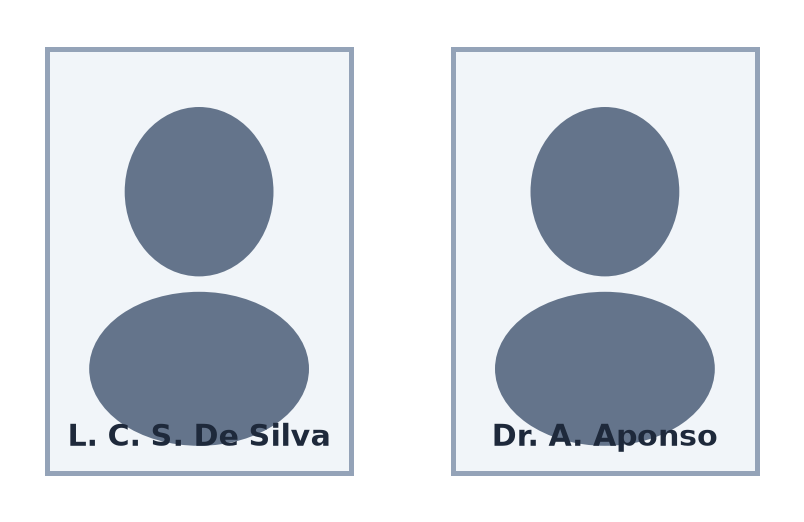
\includegraphics[width=1in,height=1.25in,clip,keepaspectratio]{figures/author1.png}}]{Laddu Chamith Shaminda De Silva}
(Graduate Student Member, IEEE) received the B.Sc. (Hons) degree in Computer Science from the Informatics Institute of Technology (IIT), Colombo, Sri Lanka, in academic partnership with the University of Westminster, London, U.K., in 2026. His research interests lie at the intersection of Explainable Artificial Intelligence (XAI), autonomous multi-agent systems, distribution-free conformal risk calibration, and cybersecurity for life-critical cyber-physical systems. He has contributed to novel epistemic verification architectures and auditable defense platforms for enterprise and clinical infrastructures.
\end{IEEEbiography}

\begin{IEEEbiography}[{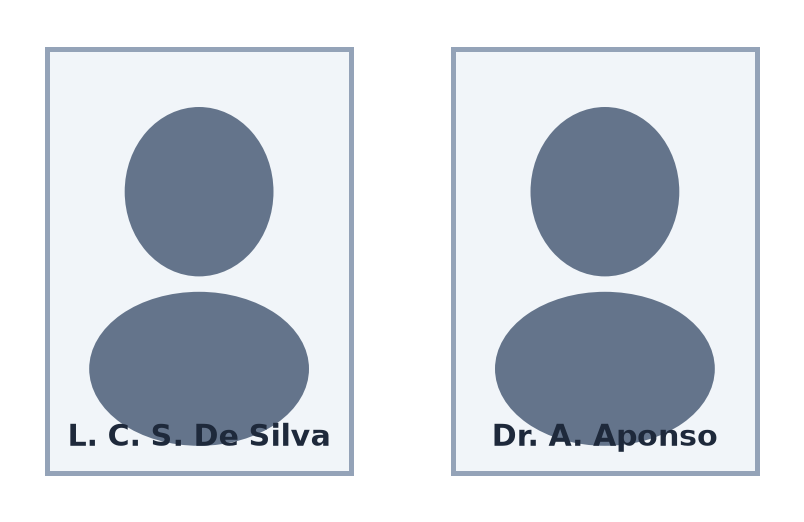
\includegraphics[width=1in,height=1.25in,clip,keepaspectratio]{figures/author2.png}}]{Aloka Aponso}
(Senior Member, IEEE) received the Ph.D. degree in Computer Science. He is currently a Senior Lecturer with the Department of Computing, Informatics Institute of Technology (IIT), Colombo, Sri Lanka. His research interests encompass machine learning, applied artificial intelligence, intelligent multi-agent systems, and automated threat reasoning. He has authored and co-authored numerous peer-reviewed research publications in international IEEE conferences and indexed journals, and actively serves as a technical reviewer and research advisor in computing systems.
\end{IEEEbiography}

\EOD

\end{document}
